% network: B(left)-A(right), 6 intermediate nodes, 10 undirected weighted edges, all solid, no arrows.
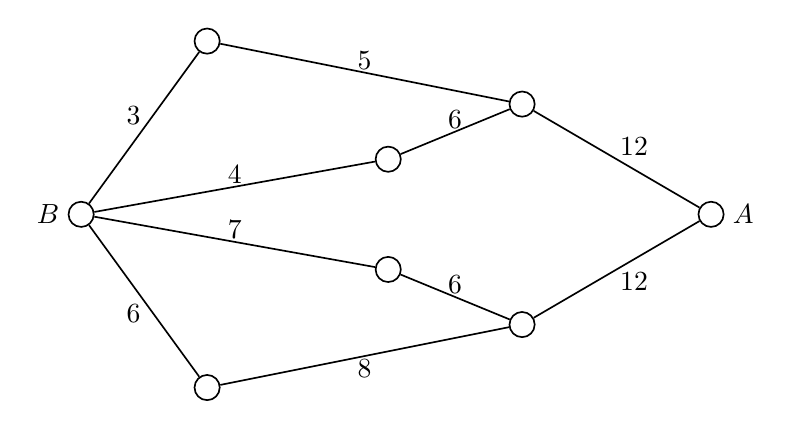
\begin{tikzpicture}[line width=.6pt,font=\normalsize,
  nd/.style={circle,draw,fill=white,minimum size=3.2mm,inner sep=0pt}]
  \node[nd] (B) at (0,0) {};
  \node[left=1.5mm] at (B) {$B$};
  \node[nd] (A) at (8,0) {};
  \node[right=1.5mm] at (A) {$A$};
  \node[nd] (nT) at (1.6,2.2) {};
  \node[nd] (nUR) at (5.6,1.4) {};
  \node[nd] (nM) at (3.9,0.7) {};
  \node[nd] (nL) at (3.9,-0.7) {};
  \node[nd] (nBR) at (5.6,-1.4) {};
  \node[nd] (nB) at (1.6,-2.2) {};
  \draw (B) -- node[above left,inner sep=1pt] {$3$} (nT);
  \draw (nT) -- node[above,inner sep=1pt] {$5$} (nUR);
  \draw (nUR) -- node[above right,inner sep=1pt] {$12$} (A);
  \draw (B) -- node[above,inner sep=1pt] {$4$} (nM);
  \draw (nM) -- node[above,inner sep=1pt] {$6$} (nUR);
  \draw (B) -- node[above,inner sep=1pt] {$7$} (nL);
  \draw (nL) -- node[above,inner sep=1pt] {$6$} (nBR);
  \draw (nBR) -- node[below right,inner sep=1pt] {$12$} (A);
  \draw (B) -- node[below left,inner sep=1pt] {$6$} (nB);
  \draw (nB) -- node[below,inner sep=1pt] {$8$} (nBR);
\end{tikzpicture}
